% The "%" character denotes a comment
% This file was written by Nathan Moore, Winona State University
% as a template for how lab reports might be written in LaTeX.
% style choices originally come from the American Journal of Physics's
% sample submission file, http://ajp.dickinson.edu/Contributors/manFormat.html
%
%
\documentclass[prb,preprint]{revtex4-1}
\usepackage{amsmath}  % needed for \tfrac, \bmatrix, etc.
\usepackage{amsfonts} % needed for bold Greek, Fraktur, and blackboard bold
\usepackage{graphicx} % needed for figures

%these are some macros (shortcuts)
\newcommand{\bea}{\begin{eqnarray}}
\newcommand{\eea}{\end{eqnarray}}
\newcommand{\be}{\begin{equation}}
\newcommand{\ee}{\end{equation}}

\begin{document}

\title{Computer Arch. Project Proposal}
\author{Adam Stammer}
%\email{adam.stammer@go.winona.edu}

\date{\today}

%if you include an abstract, it goes here
\begin{abstract}
This is a brief project proposal for my semester project in Mr. Funk's Computer Architecture class Spring semester of 2020. I aim to present the Hardware.Astronomy Housekeeping Box, a computerized electronics system designed to control and maintain the ZEUS2 astronomical spectrometer. I've worked on this project for the past seven months.
\end{abstract}

\maketitle


%These are my general reccomendations for an undergraduate lab report in Physics. 
%
%\textbf{Purpose}
%The lab report should start with a purpose statement.  Briefly 
%provide the necessary background and explain what problem your are trying to 
%solve/investigate.
%
%\textbf{Conclusions} Don't be coy, cut to the point right away and state what you found. This should be breif.
%
%\textbf{Theory} We never just measure stuff in Physics.  There's always a 
%theoretical idea behind the measurement we're making.  Explain  the ideas 
%behind your work, starting at the level of a successful Physics 221/222 
%student.
%
%\textbf{Data} Sketch out, in words and pictures, the apparatus you used to take data.  Report the data, graphically, if possible, and state the uncertainties  in your measurement.  Don't provide pages of computer printout here. Data tables shouldn't be your first choice when it comes to communicating your measurements.\cite{Tufte}
%
%\textbf{Analysis} With data presented, describe how the theory agrees/disagrees with 
%the data you took.  Normally this is accomplished with a fit line (or math 
%model) that is interpreted.
%
%\textbf{Limitations and Recommendations} Every measurement has limitations and it is only honest to report them to the reader.  ``Human Error'' is a meaningless statement.  After your analysis is complete, revisit the purpose statement.  This is the place to more forcefully argue your conclusions.    
%
%Notes: 
%Writing in the first person, eg ``I" or ``We," is fine.
%
%\newpage
%\textbf{Example Lab Report:}

\section{Why build it when you can buy something similar?}
Similar products are sold by multiple companies, so why should we spend a bunch of money designing a new system? Simple. Deprecation. It is a very very common problem, that commercial equipment outlives it's support life, or even company life. Currently, the telescope in question is using equipment sold over 30 years ago, and the company no longer exists. Thus, all hardware support for such equipment must come from the scientists themselves, which adds a new barrier of cost, time and money, to the science projects in question. The goals of this project was to alleviate that issue in more than just the ZEUS2 project. 

\section{Presentation}
I hope to present this project in a PowerPoint format, with the power hanging somewhere in the room too. If supported, I would like my presentation to be a walk-through of the problems that arose and the decisions made that have brought the project to where it is now. I think a lot of my peers have had a lacking interaction with design processes, and my hope is that this presentation can be a chance at exposing them to that. If nothing else it can help reinforce what they already know/think, but I imagine it will answer questions and start trains of thought that some people have yet to begin. The next section explains more of the project and asks just some of the questions I would like to ask and answer in my presentation.

\section{What is it?}
The poster that should accompany this document will aid in understanding the design goals of this project. In short it is a modular card based computerized system. The chassis itself hold two power supplies, BUS, Raspberry Pi, Arduino UNO, Touch Screen, and supports up to 10 cards. Each card can be designed to do whatever is needed, provided it falls within the design standards set by the project. 


Parallelization/Communication: These cards are expected to each have their own processors, along with the two processors already on the BUS. That leads to multiple conversations methods between cards, from I2C to UART and SPI. Data speeds are still a topic of worry, as for our specific implementation there will be a lot of data sharing. This is also something we cannot run ideal tests on until the board is fully built. What kind of bandwidth do we expect/measure/need?

Power Considerations: How much power is too much? Are theses power supplies easily replaced in the future? How do you get enough power without breaking the bank or putting everyone in danger? What about national power standards?

System/Human IO: How does somebody interact with the system? Turn things on or off, change settings and such?

System/System IO: How does such a system interact with the astronomical spectrometer? What kind of interactions can/need to occur.

Efficiency is another concern, both in power and in time.
\newline


There is certainly more to talk about regarding this project but I hope the above gives a satisfactory preview of how this system is indeed a computer system and the high level architecture is what I was designing, even if we never used the word "architecture" during the design process. This project is still a work in progress, which means I may very well be able to apply things learning in this class to the rest of this design, and even redesign things as needed.


%\begin{figure}[ht]
%\centering
%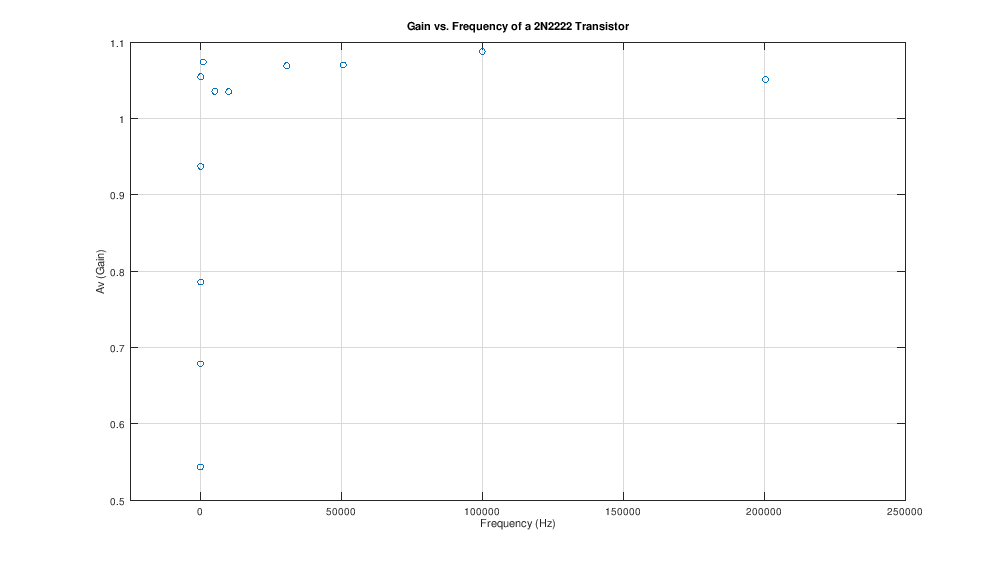
\includegraphics[width=7in]{bigGraph.png}
%\caption{This is the circuit used to take measurements. Image from NI Multisim.}
%\label{fig1}
%\end{figure}

\end{document}
